\begin{surferPage}[Sextik (30 Kuspen)]{Barths Sextik mit 30 Cuspen}
    Nachdem Wolf Barth seine Sextik mit der maximal möglichen Anzahl von $65$
    Singularitäten gefunden hatte
    und zwei seiner Doktoranden ebenfalls neue Weltrekorde für höhere Grade
    aufgestellt hatten, beschäftigt er sich auch mit der Frage nach der
    maximal möglichen Anzahl von Kuspen auf Flächen von gegebenem Grad. 

    Barths Kontruktion der Sextik mit $65$ 
    Singularitäten vom Typ $A_1^{+-}$ (also Doppelkegel) kann man auf Kuspen
    adaptieren (allerdings nur $30$ Stück):
    \[P_6 - \alpha \cdot K^3=0,\]
    wobei $P_6$ wie bei der anderen Barth-Sextik die Symmetrieebenen des
    regelmäßigen Ikosaeders sind und $K$ die Gleichung einer Kugeloberfläche
    ist:
    \vspace*{-0.4em}
    \begin{center}
      \begin{tabular}{c@{\ }c@{\ }c@{\ }c}
        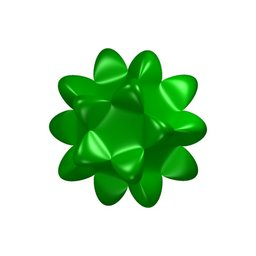
\includegraphics[height=1.2cm]{./../../common/images/barthsextic_30A2}
        &
        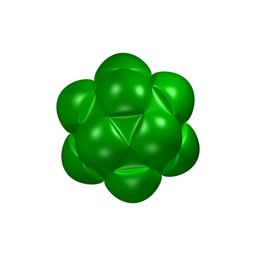
\includegraphics[height=1.2cm]{./../../common/images/barthsextic_30A2_3}
        &
        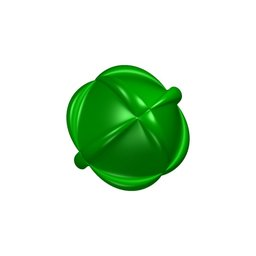
\includegraphics[height=1.2cm]{./../../common/images/barthsextic_30A2_5}
        &
        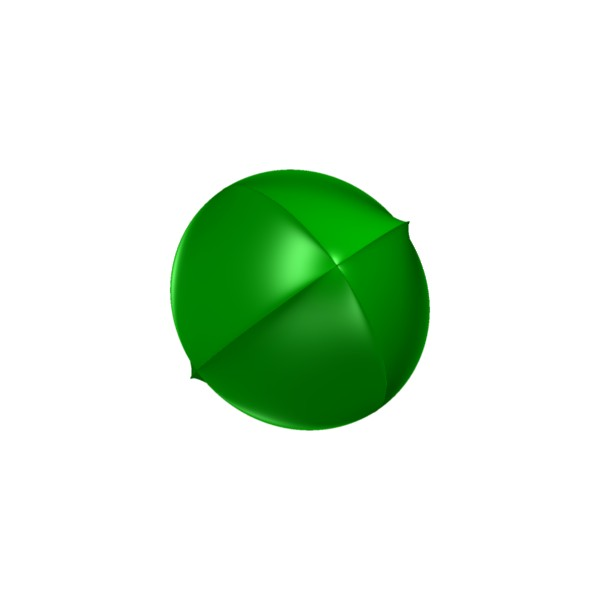
\includegraphics[height=1.2cm]{./../../common/images/barthsextic_30A2_6}
      \end{tabular}
    \end{center}    
    \vspace*{-0.3em}
    Dies ist der aktuelle Weltrekord für die maximale Anzahl reeller Kuspen
    auf Sextiken, für komplexe liegt er bei $36$.
\end{surferPage}
